% Compile with pdfLaTeX. All content, tables and the workflow are editable here.
% Source: Phase2_Report10/Phase2_Report10 (1).tex, unchanged.
\documentclass[aspectratio=169,11pt]{beamer}
\usepackage[utf8]{inputenc}
\usepackage[T1]{fontenc}
\usepackage{lmodern}
\usepackage{amsmath,amssymb,booktabs,array,graphicx,tikz}
\usetikzlibrary{arrows.meta}
\definecolor{ink}{HTML}{14314A}
\definecolor{accent}{HTML}{007F89}
\definecolor{muted}{HTML}{506371}
\setbeamercolor{normal text}{fg=ink,bg=white}
\setbeamercolor{frametitle}{fg=ink,bg=white}
\setbeamercolor{title}{fg=ink}
\setbeamercolor{structure}{fg=accent}
\setbeamercolor{alerted text}{fg=accent}
\setbeamerfont{frametitle}{size=\Large,series=\bfseries}
\setbeamerfont{title}{size=\LARGE,series=\bfseries}
\setbeamersize{text margin left=9mm,text margin right=9mm}
\setbeamertemplate{navigation symbols}{}
\setbeamertemplate{headline}{}
\setbeamertemplate{footline}{\hfill\usebeamercolor[fg]{structure}\scriptsize
  \insertframenumber\hspace{9mm}\vspace{3mm}}
\setbeamertemplate{itemize item}{\small\textbullet}
\setlength{\parskip}{6pt}
\newcolumntype{L}[1]{>{\raggedright\arraybackslash}p{#1}}
\newcommand{\smallnote}[1]{\par{\footnotesize\color{muted}#1\par}}
\title{Course Registration Helper\\for Balanced Workloads}
\subtitle{Phase 2: AI Project Presentation}
\author{}
\date{}
\hypersetup{pdftitle={Course Registration Helper for Balanced Workloads},pdfauthor={}}

\begin{document}

% 01 -- Cover
\begin{frame}[plain]
\vspace{10mm}
{\color{accent}\large Phase 2: AI Project Presentation\par}
\vspace{5mm}
{\usebeamerfont{title}Course Registration Helper\\for Balanced Workloads\par}
\vspace{7mm}
{\large Personalised course rewards and external path optimisation\par}
\end{frame}

% 02 -- Introduction
\begin{frame}{Course choices are difficult during add--drop}
\begin{itemize}\setlength{\itemsep}{7pt}
\item Students may be unfamiliar with GE and elective-course backgrounds or workloads.
\item Limited seats and newly available places can lead to rushed decisions.
\item An unsuitable choice can become difficult to reverse after add--drop.
\end{itemize}
\vspace{3mm}
Our helper uses students' interests, year and required courses to suggest suitable, workload-aware schedules.
\smallnote{It supports course selection. It does not automatically register courses or guarantee seats.}
\end{frame}

% 03 -- Data
\begin{frame}{Programme evidence becomes structured course facts}
Handbook, CM path/course list, CS major and suggested plan, GE information, and saved Semester A/B timetables.
\vspace{2mm}
\begin{tabular}{L{9.4cm}r}
\toprule
Timetable PDFs collected & 93\\
Successfully parsed / excluded & 86 / 7\\
Timetable PDFs represented in programme training & 82\\
Programme PDFs represented in programme training & 3\\\midrule
\textbf{PDF sources represented in the 485-example split} & \textbf{85}\\
\bottomrule
\end{tabular}\par
\vspace{2mm}
We train on extracted text and facts as JSON: course identities, credits, prerequisites, exclusions, restrictions and meetings.
\smallnote{The count covers this programme-training split. Earlier handbook, GE and study-path stages are outside it. Sources: supplied CityUHK documents.}
\end{frame}

% 04 -- Fine tuning and prompts
\begin{frame}{Qwen learns a structured reward policy}
Qwen3-8B uses rank-8 QLoRA, a frozen four-bit base and BF16 computation.
\vspace{1mm}
\begin{tabular}{L{7.5cm}L{4.8cm}}
\toprule
Training stage & Examples\\\midrule
Programme data & 485 train / 24 validation / 30 test\\
CM background update & 244 / 32, plus 20 held-out checks\\
Relation distillation & 149 / 20\\
Maximum-versus-sum correction & 82 corrective examples\\
\bottomrule
\end{tabular}\par
\vspace{2mm}
Prompts combine system instructions with student facts/states. Assistant JSON targets use assistant-only cross-entropy loss.
\smallnote{The current prompt allows only \texttt{reward\_parameters} and \texttt{course\_relations}. One local inference exported all eight settings and 26 links without fallback. This tests policy export, not independent reward quality.}
\end{frame}

% 05 -- Workflow, retaining the report's human feedback loop
\begin{frame}{GPT teaches rewards; a tool selects the path}
\centering
\resizebox{\linewidth}{!}{%
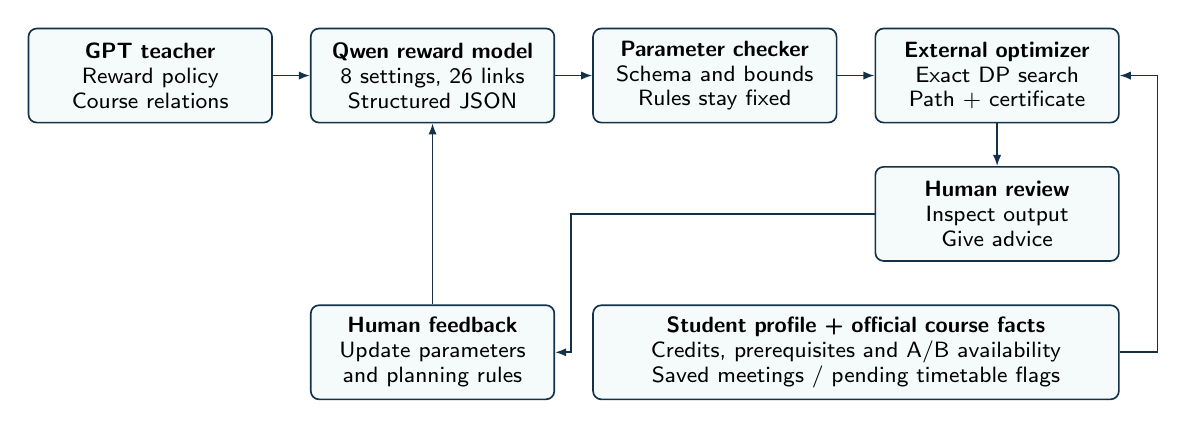
\begin{tikzpicture}[
 x=1pt,y=1pt,
 flowbox/.style={draw=ink,fill=accent!4,rounded corners=3pt,
 line width=.6pt,align=center,text width=82pt,minimum height=34pt,
 inner sep=3pt,font=\sffamily\fontsize{8}{9}\selectfont},
 flowarrow/.style={-{Latex[length=4pt,width=3pt]},draw=ink,line width=.6pt}]
\node[flowbox] (teacher) at (47,117)
 {\textbf{GPT teacher}\\Reward policy\\Course relations};
\node[flowbox] (qwen) at (149,117)
 {\textbf{Qwen reward model}\\8 settings, 26 links\\Structured JSON};
\node[flowbox] (checker) at (251,117)
 {\textbf{Parameter checker}\\Schema and bounds\\Rules stay fixed};
\node[flowbox] (optimizer) at (353,117)
 {\textbf{External optimizer}\\Exact DP search\\Path + certificate};
\draw[flowarrow] (teacher.east)--(qwen.west);
\draw[flowarrow] (qwen.east)--(checker.west);
\draw[flowarrow] (checker.east)--(optimizer.west);
\node[flowbox] (human) at (353,67)
 {\textbf{Human review}\\Inspect output\\Give advice};
\node[flowbox] (feedback) at (149,17)
 {\textbf{Human feedback}\\Update parameters\\and planning rules};
\node[flowbox,text width=184pt] (facts) at (302,17)
 {\textbf{Student profile + official course facts}\\
 Credits, prerequisites and A/B availability\\Saved meetings / pending timetable flags};
\draw[flowarrow] (feedback.north)--(qwen.south);
\draw[flowarrow] (optimizer.south)--(human.north);
\draw[flowarrow] (human.west)--(199,67)--(199,17)--(feedback.east);
\draw[flowarrow] (facts.east)--(411,17)--(411,117)--(optimizer.east);
\end{tikzpicture}}
\vspace{3mm}
\raggedright
GPT teaches course relations and rewards. Fictional examples and human advice guide retraining or planning-rule updates after output review.
\end{frame}

% 06 -- Hardware
\begin{frame}{Local training and inference fit on one RTX 5090}
\textbf{NVIDIA GeForce RTX 5090: 31.82 GiB total CUDA device memory.}
\vspace{1mm}
\begin{tabular}{L{9cm}r}
\toprule
Separate training run & Peak allocated GiB\\\midrule
Programme training & 8.27\\
Finance-background update & 7.37\\
Relation correction & 8.35\\
Longer-context degree-policy update & 15.84\\\midrule
Representative inference & 5.99\\
\bottomrule
\end{tabular}\par
\smallnote{Training: one example per microbatch, accumulation over four examples, 4,096-token contexts (6,144 for degree policy). Inference: batch 1, 598-token prompt, 33-token response; loaded allocation 5.74 GiB and peak reserved 6.10 GiB. Measurements cover this process's PyTorch memory, excluding other apps and driver memory. Context and batch size affect consumption. Python path search runs on CPU.}
\end{frame}

% 07 -- Hard constraints
\begin{frame}{The whole path must satisfy the degree audit}
\begin{itemize}\setlength{\itemsep}{5pt}
\item At least \textbf{122 unique credits}, also satisfying 121.
\item Four distributional GEs covering Areas 1--3, with at most one per semester. Compulsory language/development GE is separate.
\item At least 20 elective mathematics credits outside core/capstone study.
\item Mandatory/core courses, project, free electives and chosen stream complete.
\item Each term has zero to six positive-credit courses and at most 18 credits.
\end{itemize}
\smallnote{Courses must appear in the student's designated programme document or the verified GE collection. High reward cannot compensate for missing required credits.}
\end{frame}

% 08 -- Penalty becomes reward
\begin{frame}{The original penalties become part of net reward}
Original weighted penalty for binary course choices $x_i$:
\[
\min_{\mathbf x\in\mathcal X}P(\mathbf x),\qquad
P(\mathbf x)=\sum_i x_i(\lambda_b b_i+\lambda_d d_i+\lambda_w w_i).
\]
Adding course value $R_i$ gives the net-reward objective:
\[
\max_{\mathbf x\in\mathcal X}\left[\sum_i x_iR_i-P(\mathbf x)\right].
\]
\vspace{1mm}
Students adjust non-negative weights for background mismatch ($\lambda_b$), difficulty ($\lambda_d$) and workload ($\lambda_w$).
\smallnote{Degree constraints $\mathcal X$ remain binding. Higher penalty lowers reward.}
\end{frame}

% 09 -- State dependent reward
\begin{frame}{Rewards change with completed study and stream progress}
\begin{align*}
U(X,s)={}&\sum_{c\in X}\bigl[g_c(s)+p_c(s)+h_c(s)+q_c(s)+z_c(s)\\
 &-\lambda_b(b_c(s)+e_c(s))-\lambda_d d_c(s)-\lambda_w w_c(s)\bigr]\\
 &+R_{\mathrm{stream}}(X,s)-O(X,s).
\end{align*}
\begin{tabular}{L{6.2cm}L{6cm}}
$g$: base course value & $p$: preparation from earlier study\\
$h$: core priorities & $q$: prerequisite bridges\\
$z$: quota/timing bonuses & $R_{\mathrm{stream}}$: stream progress\\
\end{tabular}\par
\vspace{2mm}
Claiming one selected stream earns 6 once, multiplied by the student's stream weight.
\smallnote{These scores are configured estimates, not measured study hours.}
\end{frame}

% 10 -- Overload
\begin{frame}{Overload starts above 15 credits, or 12 in Year 4}
\[
O(X,s)=\begin{cases}
0.25[\max(0,C(X)-15)]^2,&\text{Years 1--3},\\[6pt]
0.25[\max(0,C(X)-12)]^2,&\text{Year 4}.
\end{cases}
\]
\vspace{3mm}
The 18-credit maximum remains a separate hard constraint.

Term loads stay flexible. A 12- or 13-credit term is valid when the full path reaches 122 credits and satisfies the degree audit.
\smallnote{There is no five-course minimum in every term.}
\end{frame}

% 11 -- Optimisation program
\begin{frame}{Python dynamic programming finds the largest reward}
\begin{enumerate}\setlength{\itemsep}{7pt}
\item Start with completed courses and fixed allocations.
\item Explore permitted semester placements of remaining courses.
\item Update student state in semester order and calculate total discounted reward.
\item Merge identical partial allocations to avoid repeated calculations.
\item Compare feasible completions and return the largest objective value.
\end{enumerate}
\smallnote{The maximum applies to the supplied choices. Qwen provides validated parameters and relations; the external program performs path selection. The latest optimiser revision did not retrain neural weights.}
\end{frame}

% 12 -- Blind test profiles
\begin{frame}{Three fictional profiles form the blind comparison}
Each student passes exactly 15 credits in Year 1A and 15 in Year 1B.
\vspace{1mm}
\begin{tabular}{lL{3cm}L{3cm}L{4cm}}
\toprule
Profile & Year 1A GE & Year 1B GE & Desired stream\\\midrule
F & GE2260, Area 2 & GE1105, Area 1 & Financial Mathematics\\[4pt]
N & GE1305, Area 3 & GE1113, Area 1 & Financial Mathematics\\[4pt]
M & GE2134, Area 1 & GE1305, Area 3 & Enriched Mathematics\\
\bottomrule
\end{tabular}\par
\vspace{2mm}
\smallnote{Common Year 1A: MA1300, CS1302, PHY1201, GE1401. Common Year 1B: MA1301, CHEM1200, GE1501, GE2401. Each term adds the profile-specific GE above.}
\smallnote{Within each case, both methods receive the same history and fixed future context. Context differs across cases, so this is not a causal comparison of GE histories.}
\end{frame}

% 13 -- Comparison results
\begin{frame}{Both methods choose the same six elective placements}
\small
\begin{tabular}{lL{5.5cm}L{5.5cm}}
\toprule
 & Qwen rewards + external DP & Direct GPT, without optimiser\\\midrule
F & Y3B: MA4529, MA4537\newline Y4A: MA4528\newline Y4B: MA4546, MA4550, MA4551 & Y3B: MA4529, MA4537\newline Y4A: MA4528\newline Y4B: MA4546, MA4550, MA4551\\[5pt]
N & Y3A: MA4528\newline Y4B: MA4529, MA4537, MA4546, MA4550, MA4551 & Y3A: MA4528\newline Y4B: MA4529, MA4537, MA4546, MA4550, MA4551\\[5pt]
M & Y3B: MA4537, MA4546\newline Y4A: MA4528\newline Y4B: MA4529, MA4550, MA4551 & Y3B: MA4537, MA4546\newline Y4A: MA4528\newline Y4B: MA4529, MA4550, MA4551\\
\bottomrule
\end{tabular}\par
\vspace{2mm}
\normalsize Both methods pass the encoded curriculum audit in all three cases and reach the same certified completion optimum.
\end{frame}

% 14 -- Protocol
\begin{frame}{The baseline selects placements without optimisation tools}
\begin{itemize}\setlength{\itemsep}{7pt}
\item Direct GPT receives the same parameter packet and course facts.
\item GPT uses no solver, code or browsing, and sees no optimiser answers or scores.
\item A common critic checks the final outputs, with no repair or fallback for GPT.
\item An omitted state-dependent cost was corrected before the final comparison. Pilot outputs were excluded.
\end{itemize}
\smallnote{The exact comparator endpoint is unverified, so the report labels it GPT. The evaluation uses familiar evidence, fictional transcripts and synthetic policies, rather than real workload or unseen-cohort generalisation.}
\end{frame}

% 15 -- Full path first half
\begin{frame}{Profile N reaches 64 credits after Year 2}
\small
\begin{tabular}{lL{9.3cm}rr}
\toprule
Term & Courses & CUs & Total\\\midrule
Y1A & MA1300, CS1302, PHY1201, GE1401, GE1305 & 15 & 15\\[7pt]
Y1B & MA1301, CHEM1200, GE1501, GE2401, GE1113 & 15 & 30\\[7pt]
Y2A & CS2360, CSCI1001$^{*}$ (0), GE1601$^{*}$, GE2260, MA2503, MA2508, MA2509 & 18 & 48\\[7pt]
Y2B & CS2468, CSCI1002$^{*}$ (0), EF3320, MA2507, MA3511, MA3515, MA3517 & 16 & 64\\
\bottomrule
\end{tabular}\par
\vspace{3mm}
\normalsize The Year-1 history stays unchanged. All future grades are assumed passes for this simulation.
\smallnote{A star marks pending class details. Zero-credit catch-up tasks require confirmation. Both methods produce the same full path.}
\end{frame}

% 16 -- Full path second half
\begin{frame}{Profile N finishes the projected path at 122 credits}
\small
\begin{tabular}{lL{9.3cm}rr}
\toprule
Term & Courses & CUs & Total\\\midrule
Y3A & GE1105, MA3512, MA3525, MA4528$^{*}$, MA4545 & 15 & 79\\[6pt]
Y3B & MA2510, MA3514, MA3523, MA3526, MA3530 & 13 & 92\\[6pt]
Y4A & MA3518, MA3521, MA4530 (A)$^{*}$, MA4542 & 12 & 104\\[6pt]
Y4B & MA4529$^{*}$, MA4530 (B)$^{*}$, MA4537$^{*}$, MA4546$^{*}$, MA4550$^{*}$, MA4551$^{*}$ & 18 & 122\\
\bottomrule
\end{tabular}\par
\vspace{2mm}
\normalsize All three paths contain four GEs across Areas 1--3, 30 elective mathematics credits, 45 core credits and six project credits.
\smallnote{25 future credits lack saved class details and retain null meetings/CRNs. MA4530 parts form one six-credit year-long project, split three credits per term. Curriculum completion remains distinct from confirmed registration. Profile N's final term incurs a nine-point overload penalty.}
\end{frame}

% 17 -- Parameter sensitivity
\begin{frame}{Changing an overload weight changes the selected path}
Profile F keeps the same history and course relations. Only the Year-4 overload coefficient changes.
\vspace{4mm}
\begin{tabular}{L{5.7cm}rrr}
\toprule
Year-4 coefficient & Year 3B CUs & Year 4B CUs & Total\\\midrule
0.25, configured & 18 & 15 & 122\\[6pt]
0, counterfactual & 15 & 18 & 122\\
\bottomrule
\end{tabular}\par
\vspace{4mm}
The optimiser responds to supplied parameters rather than reproducing a fixed language-model answer.
\smallnote{The configured policy remains 0.25. The zero-weight run is a controlled counterfactual.}
\end{frame}

% 18 -- Dependency table
\begin{frame}{Earlier study changes specific course rewards}
\small
\begin{tabular}{L{6.3cm}L{2cm}L{3.5cm}}
\toprule
Changed history or preference & Target & Reward effect\\\midrule
Pass MA2508 & MA3515 & Preparation $+0.20$\\[6pt]
Pass MA2509 & GE2134 & Preparation $+0.15$\\[6pt]
Covered Area 1 replaces Area 2 & GE1113 & Base reward $-2.70$\\[6pt]
Pass GE2260; finance selected & MA3521 & Stream reward $+4.00$\\[6pt]
Pass MA2503; portfolio mathematics & EF3320 & Preparation $+0.20$\\
\bottomrule
\end{tabular}\par
\vspace{3mm}
\normalsize Twelve paired interventions match their predeclared policy effects.
\smallnote{Year, base profit, score vector and penalty weights stay fixed, excluding credit-progress and overload effects. These test configured mechanisms, rather than empirical learning benefits.}
\end{frame}

% 19 -- Discussion of local model
\begin{frame}{A local reward model supports reuse and personal input}
\begin{itemize}\setlength{\itemsep}{8pt}
\item \textbf{Transfer learning:} a larger teacher helps a smaller model produce similar recommendations in the reported examples.
\item \textbf{Privacy:} local transcript processing avoids sending that personal input over the internet to GPT.
\item \textbf{Updates:} a shared fine-tuned model reduces repeated manual provision of course data as semesters change.
\item \textbf{Deployment:} the small model can act as a module in a course-advice chatbot.
\end{itemize}
\end{frame}

% 20 -- Discussion of possible simplification
\begin{frame}{A fixed input format could simplify the model component}
The report considers storing finite course relations and state-dependent parameters in a database.

With fixed inputs, a simpler encoder or script could replace the LLM component.

The report also discusses reducing candidate paths using known course chains, such as GE2340 leading towards machine learning.
\smallnote{This is a possible simplification discussed in the report. The implemented path-selection method presented here is exact dynamic programming over the supplied choices.}
\end{frame}

% 21 -- Limitations and conclusion
\begin{frame}{Further student evidence can improve the reward policy}
\begin{itemize}\setlength{\itemsep}{6pt}
\item Teacher advice and personal feedback do not cover first-hand experience of every course.
\item Workload estimates need student feedback and information about teaching requirements.
\item Venue and inconvenient daily arrangements remain possible additions to the reward function.
\end{itemize}
\vspace{3mm}
\textbf{Our helper combines LLM-generated rewards and relations with external dynamic programming for personalised study-path selection.}
\smallnote{The reported tests show potential for the method. More evidence and richer decision factors are needed to make the helper more complete.}
\end{frame}

% 22 -- References retained from the report
\begin{frame}{References}
\small
\textbf{Qwen3}\par
A. Yang et al., \emph{Qwen3 Technical Report}, 2025.\\
\url{https://arxiv.org/abs/2505.09388}\par
\vspace{3mm}
\textbf{QLoRA}\par
T. Dettmers et al., \emph{QLoRA: Efficient Finetuning of Quantized LLMs}, 2023.\\
\url{https://arxiv.org/abs/2305.14314}\par
\vspace{3mm}
\textbf{CityUHK supplied documents}\par
Student Handbook 2026--27, CM 2025-entry path/course list, CS major/suggested plan, GE information and saved Semester A/B timetables. Advanced-course rules include:\\
\url{https://www.cityu.edu.hk/catalogue/ug/current/course/MA4537.htm}
\end{frame}

\end{document}
